\documentclass[10pt,a4paper]{article}
\usepackage[UTF8,fontset = windows]{ctex}
\setCJKmainfont[BoldFont=黑体,ItalicFont=楷体]{华文中宋}
\usepackage{amssymb,amsmath,amsfonts,amsthm,mathrsfs,dsfont,graphicx}
\usepackage{ifthen,indentfirst,enumerate,color,titletoc}
\usepackage{tikz}
\usepackage{multicol}
\usepackage{makecell}
\usepackage{longtable}
\usetikzlibrary{arrows,calc,intersections,patterns,decorations.pathreplacing,3d,angles,quotes}
\usepackage[bf,small,indentafter,pagestyles]{titlesec}
\usepackage[top=1in, bottom=1in,left=0.8in,right=0.8in]{geometry}
\renewcommand{\baselinestretch}{1.65}
\newtheorem{defi}{定义~}
\newtheorem{eg}{例~}
\newtheorem{ex}{~}
\newtheorem{rem}{注~}
\newtheorem{thm}{定理~}
\newtheorem{coro}{推论~}
\newtheorem{axiom}{公理~}
\newtheorem{prop}{性质~}
\newcommand{\blank}[1]{\underline{\hbox to #1pt{}}}
\newcommand{\bracket}[1]{(\hbox to #1pt{})}
\newcommand{\onech}[4]{\par\begin{tabular}{p{.9\textwidth}}
A.~#1\\
B.~#2\\
C.~#3\\
D.~#4
\end{tabular}}
\newcommand{\twoch}[4]{\par\begin{tabular}{p{.46\textwidth}p{.46\textwidth}}
A.~#1& B.~#2\\
C.~#3& D.~#4
\end{tabular}}
\newcommand{\vartwoch}[4]{\par\begin{tabular}{p{.46\textwidth}p{.46\textwidth}}
(1)~#1& (2)~#2\\
(3)~#3& (4)~#4
\end{tabular}}
\newcommand{\fourch}[4]{\par\begin{tabular}{p{.23\textwidth}p{.23\textwidth}p{.23\textwidth}p{.23\textwidth}}
A.~#1 &B.~#2& C.~#3& D.~#4
\end{tabular}}
\newcommand{\varfourch}[4]{\par\begin{tabular}{p{.23\textwidth}p{.23\textwidth}p{.23\textwidth}p{.23\textwidth}}
(1)~#1 &(2)~#2& (3)~#3& (4)~#4
\end{tabular}}
\begin{document}
\begin{enumerate}[1.]
\item 123
\end{enumerate}

\begin{center}
\begin{tabular}{|p{.1\textwidth}<{\centering}|p{.2\textwidth}<{\centering}|p{.2\textwidth}<{\centering}|p{.2\textwidth}<{\centering}|p{.2\textwidth}<{\centering}|}
\hline
图示 & 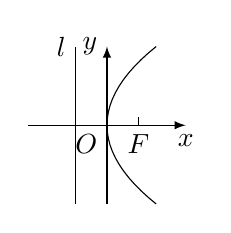
\begin{tikzpicture}[>=latex] 
\draw [->] (-1,0) -- (1,0) node [below] {$x$};
\draw [->] (0,-1) -- (0,1) node [left] {$y$};
\draw (0,0) node [below left] {$O$};
\draw (-0.4,-1) -- (-0.4,1) node [left] {$l$};
\draw (0.4,0.1) -- (0.4,0) node [below] {$F$};
\draw [domain = -1:1] plot ({pow(\x,2)/1.6},\x);
\end{tikzpicture} & 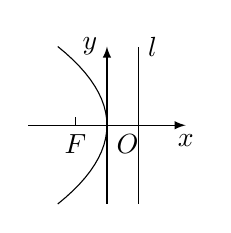
\begin{tikzpicture}[>=latex] 
\draw [->] (-1,0) -- (1,0) node [below] {$x$};
\draw [->] (0,-1) -- (0,1) node [left] {$y$};
\draw (0,0) node [below right] {$O$};
\draw (0.4,-1) -- (0.4,1) node [right] {$l$};
\draw (-0.4,0.1) -- (-0.4,0) node [below] {$F$};
\draw [domain = -1:1] plot ({-pow(\x,2)/1.6},\x);
\end{tikzpicture} &  & \\ \hline
标准方程 & $y^2=2px$($p>0$) & & $x^2=2py$($p>0$) & \\ \hline
焦点坐标 & $(\dfrac p2,0)$ & & & $(0,-\dfrac p2)$ \\ \hline
准线方程 & $x=-\dfrac p2$ & & & $y=\dfrac p2$ \\ \hline
\end{tabular}
\end{center}

\begin{center}
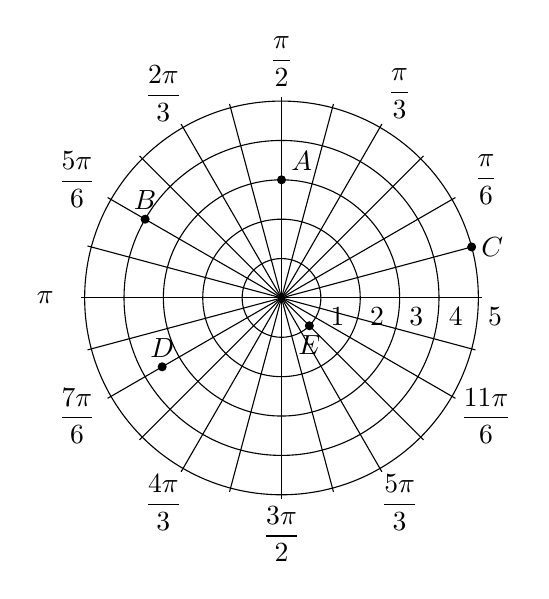
\begin{tikzpicture}[>=latex,scale = 0.5]
\foreach \i in {0,15,...,345} {\draw (0,0) -- (\i:5.1);};
\foreach \i in {1,2,...,5} {\draw (0,0) circle (\i); \draw (\i,0) node [below right] {$\i$};};
\draw (30:6) node {$\dfrac \pi 6$};
\draw (60:6) node {$\dfrac \pi 3$};
\draw (90:6) node {$\dfrac \pi 2$};
\draw (120:6) node {$\dfrac {2\pi} 3$};
\draw (150:6) node {$\dfrac {5\pi} 6$};
\draw (180:6) node {$\pi$};
\draw (210:6) node {$\dfrac {7\pi} 6$};
\draw (240:6) node {$\dfrac {4\pi} 3$};
\draw (270:6) node {$\dfrac {3\pi} 2$};
\draw (300:6) node {$\dfrac {5\pi} 3$};
\draw (330:6) node {$\dfrac {11\pi} 6$};
\filldraw (90:3) circle (0.1) node [above right] {$A$};
\filldraw (150:4) circle (0.1) node [above] {$B$};
\filldraw (15:5) circle (0.1) node [right] {$C$};
\filldraw (210:3.5) circle (0.1) node [above] {$D$};
\filldraw (315:1) circle (0.1) node [below] {$E$};
\end{tikzpicture}
\end{center}

\begin{center}
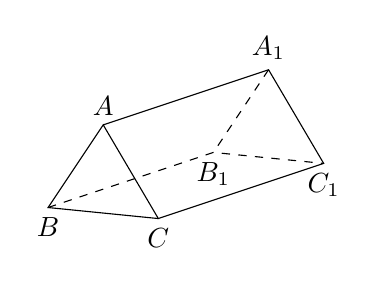
\begin{tikzpicture}[>=latex,scale = 0.7]
\draw (0,0) node [below] {$B$} coordinate (B);
\draw (2,-0.2) node [below] {$C$} coordinate (C);
\draw (1,1.5)  node [above] {$A$} coordinate (A);
\draw (A) ++ (3,1) node [above] {$A_1$} coordinate (A1);
\draw (B) ++ (3,1) node [below] {$B_1$} coordinate (B1);
\draw (C) ++ (3,1) node [below] {$C_1$} coordinate (C1);
\draw (B) -- (C) -- (A) -- cycle (C) -- (C1) -- (A1) -- (A);
\draw [dashed] (B) -- (B1) -- (C1) (A1) -- (B1);
\end{tikzpicture}
\end{center}

\begin{center}
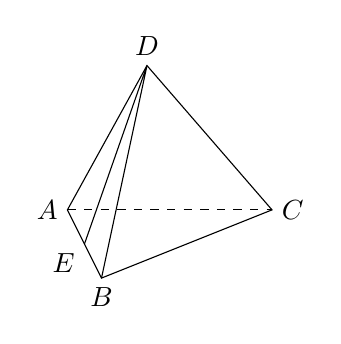
\begin{tikzpicture}[>=latex,scale = 1.5]
\draw ({sqrt(3)/2},0,-0.5) node [right] {$C$} coordinate (C);
\draw ({-sqrt(3)/2},0,-0.5) node [left] {$A$} coordinate (A);
\draw (0,0,1)  node [below] {$B$} coordinate (B);
\draw (0,{sqrt(2)},0)  node [above] {$D$} coordinate (D);
\draw (A) -- (B) -- (C) -- (D) -- cycle;
\draw ($(A)!0.5!(B)$) node [below left] {$E$} -- (D) (B) -- (D);
\draw [dashed] (A) -- (C);
\end{tikzpicture}
\end{center}

\begin{center}
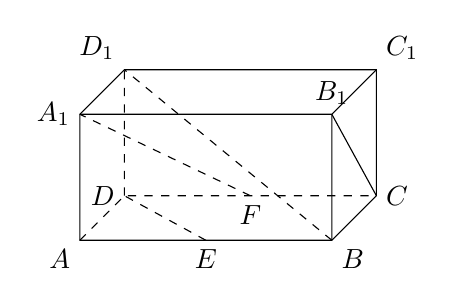
\begin{tikzpicture}[>=latex,scale = 0.8]
\draw (0,0) node [below left] {$A$} coordinate (A) --++ (4,0) node [below right] {$B$} coordinate (B) --++ (45:{2/2}) node [right] {$C$} coordinate (C)
--++ (0,2) node [above right] {$C_1$} coordinate (C1)
--++ (-4,0) node [above left] {$D_1$} coordinate (D1) --++ (225:{2/2}) node [left] {$A_1$} coordinate (A1) -- cycle;
\draw (A) ++ (4,2) node [above] {$B_1$} coordinate (B1) -- (B) (B1) --++ (45:{2/2}) (B1) --++ (-4,0);
\draw [dashed] (A) --++ (45:{2/2}) node [left] {$D$} coordinate (D) --++ (4,0) (D) --++ (0,2);
\draw [dashed] ($(A)!0.5!(B)$) node [below] {$E$} -- (D) ($(C)!0.5!(D)$) node [below] {$F$} -- (A1) (B) -- (D1);
\draw (B1) -- (C);
\end{tikzpicture}
\end{center}

\begin{center}
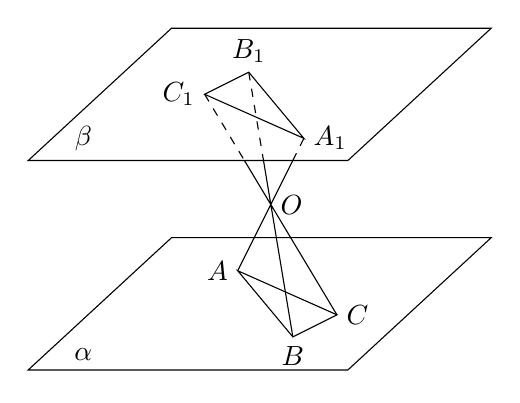
\begin{tikzpicture}[>=latex,scale = 1.4]
\draw (0.4,0.5) --++ (2.9,0) --++ (1.3,1.2) --++ (-2.9,0) -- cycle;
\draw [name path = ceiling] (0.4,0.5) ++ (0,1.9) --++ (2.9,0) --++ (1.3,1.2) --++ (-2.9,0) -- cycle;
\draw (0.9,0.5) node [above] {$\alpha$} (0.9,2.4) node [above] {$\beta$};
\draw (2.6,2) node [right] {$O$} coordinate (O);
\draw (2.3,1.4) node [left] {$A$} coordinate (A);
\draw (2.8,0.8) node [below] {$B$} coordinate (B);
\draw (3.2,1) node [right] {$C$} coordinate (C);
\path [name path = OA] (A) -- ($(A)!2!(O)$) node [right] {$A_1$} coordinate (A1);
\path [name path = OB] (B) -- ($(B)!2!(O)$) node [above] {$B_1$} coordinate (B1);
\path [name path = OC] (C) -- ($(C)!2!(O)$) node [left] {$C_1$} coordinate (C1);
\path [name intersections = {of = OA and ceiling, by = A2}];
\path [name intersections = {of = OB and ceiling, by = B2}];
\path [name intersections = {of = OC and ceiling, by = C2}];
\draw (A) -- (A2) (B) -- (B2) (C) -- (C2);
\draw [dashed] (A1) -- (A2) (B1) -- (B2) (C1) -- (C2);
\draw (A) -- (B) -- (C) -- cycle (A1) -- (B1) -- (C1) -- cycle;
\end{tikzpicture}
\end{center}

\begin{center}
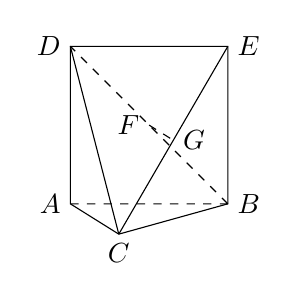
\begin{tikzpicture}[>=latex]
\draw (0,0,0) node [left] {$A$} coordinate (A);
\draw (2,0,0) node [right] {$B$} coordinate (B);
\draw (1,0,1) node [below] {$C$} coordinate (C);
\draw (A) ++ (0,2) node [left] {$D$} coordinate (D);
\draw (B) ++ (0,2) node [right] {$E$} coordinate (E);
\draw (A) -- (C) -- (B) -- (E) -- (D) -- cycle;
\draw (C) -- (D) (C) -- (E);
\draw [dashed] (A) -- (B) (B) -- (D);
\draw [dashed] ($(B)!0.5!(D)$) node [left] {$F$} -- ($(C)!0.5!(E)$) node [right] {$G$};
\end{tikzpicture}
\end{center}

\begin{center}
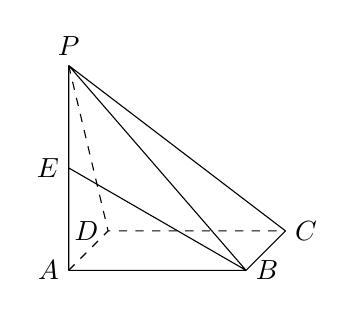
\begin{tikzpicture}[>=latex,scale = 1.3]
\draw (0,0,0) node [left] {$A$} coordinate (A);
\draw ({sqrt(3)},0,0) node [right] {$B$} coordinate (B);
\draw (B) ++ (0,0,-1) node [right] {$C$} coordinate (C);
\draw (A) ++ (0,0,-1) node [left] {$D$} coordinate (D);
\draw (A) ++ (0,2,0) node [above] {$P$} coordinate (P);
\draw ($(A)!0.5!(P)$) node [left] {$E$} coordinate (E);
\draw (P) -- (A) (P) -- (B) (P) -- (C) (A) -- (B) -- (C) (E) -- (B);
\draw [dashed] (A) -- (D) -- (C) (P) -- (D);
\end{tikzpicture}
\end{center}

\begin{center}
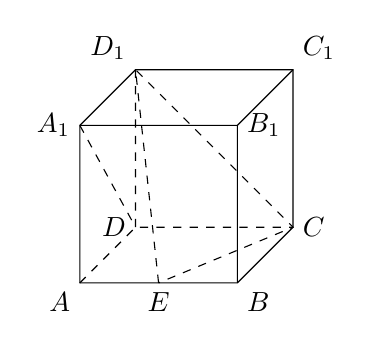
\begin{tikzpicture}[>=latex]
\draw (0,0) node [below left] {$A$} coordinate (A) --++ (2,0) node [below right] {$B$} coordinate (B) --++ (45:{2/2}) node [right] {$C$} coordinate (C)
--++ (0,2) node [above right] {$C_1$} coordinate (C1)
--++ (-2,0) node [above left] {$D_1$} coordinate (D1) --++ (225:{2/2}) node [left] {$A_1$} coordinate (A1) -- cycle;
\draw (A) ++ (2,2) node [right] {$B_1$} coordinate (B1) -- (B) (B1) --++ (45:{2/2}) (B1) --++ (-2,0);
\draw [dashed] (A) --++ (45:{2/2}) node [left] {$D$} coordinate (D) --++ (2,0) (D) --++ (0,2);
\draw ($(A)!0.5!(B)$) node [below] {$E$} coordinate (E);
\draw [dashed] (E) -- (D1) -- (C) -- cycle (A1) -- (D);
\end{tikzpicture}
\end{center}


\end{document}